% 问题重述
\section{问题重述}
\label{sec:background}

\subsection{问题背景}

2026 年 7 月，广西横州市镇龙乡遭受严重洪涝灾害，道路与桥梁损毁，多处村屯
成为与外界隔绝的孤岛\cite{refXinhua,refXinhua2}。应急物资只能依赖无人机从
调度中心 O01 空运至各受灾服务区。镇龙乡属典型山区地形，山峰与沟谷高差达数百
米，低空飞行易被山体遮挡，无人机与调度中心之间的无线电通信难以全程保持视距
链路，成为应急投送的关键瓶颈。图 \ref{fig:map} 给出研究区域内的数字高程模型
与调度节点分布，可见 O01 与 S001 至 S015 共 15 个服务区散布于河谷与山脊之间。

\begin{figure}[htbp]
\centering
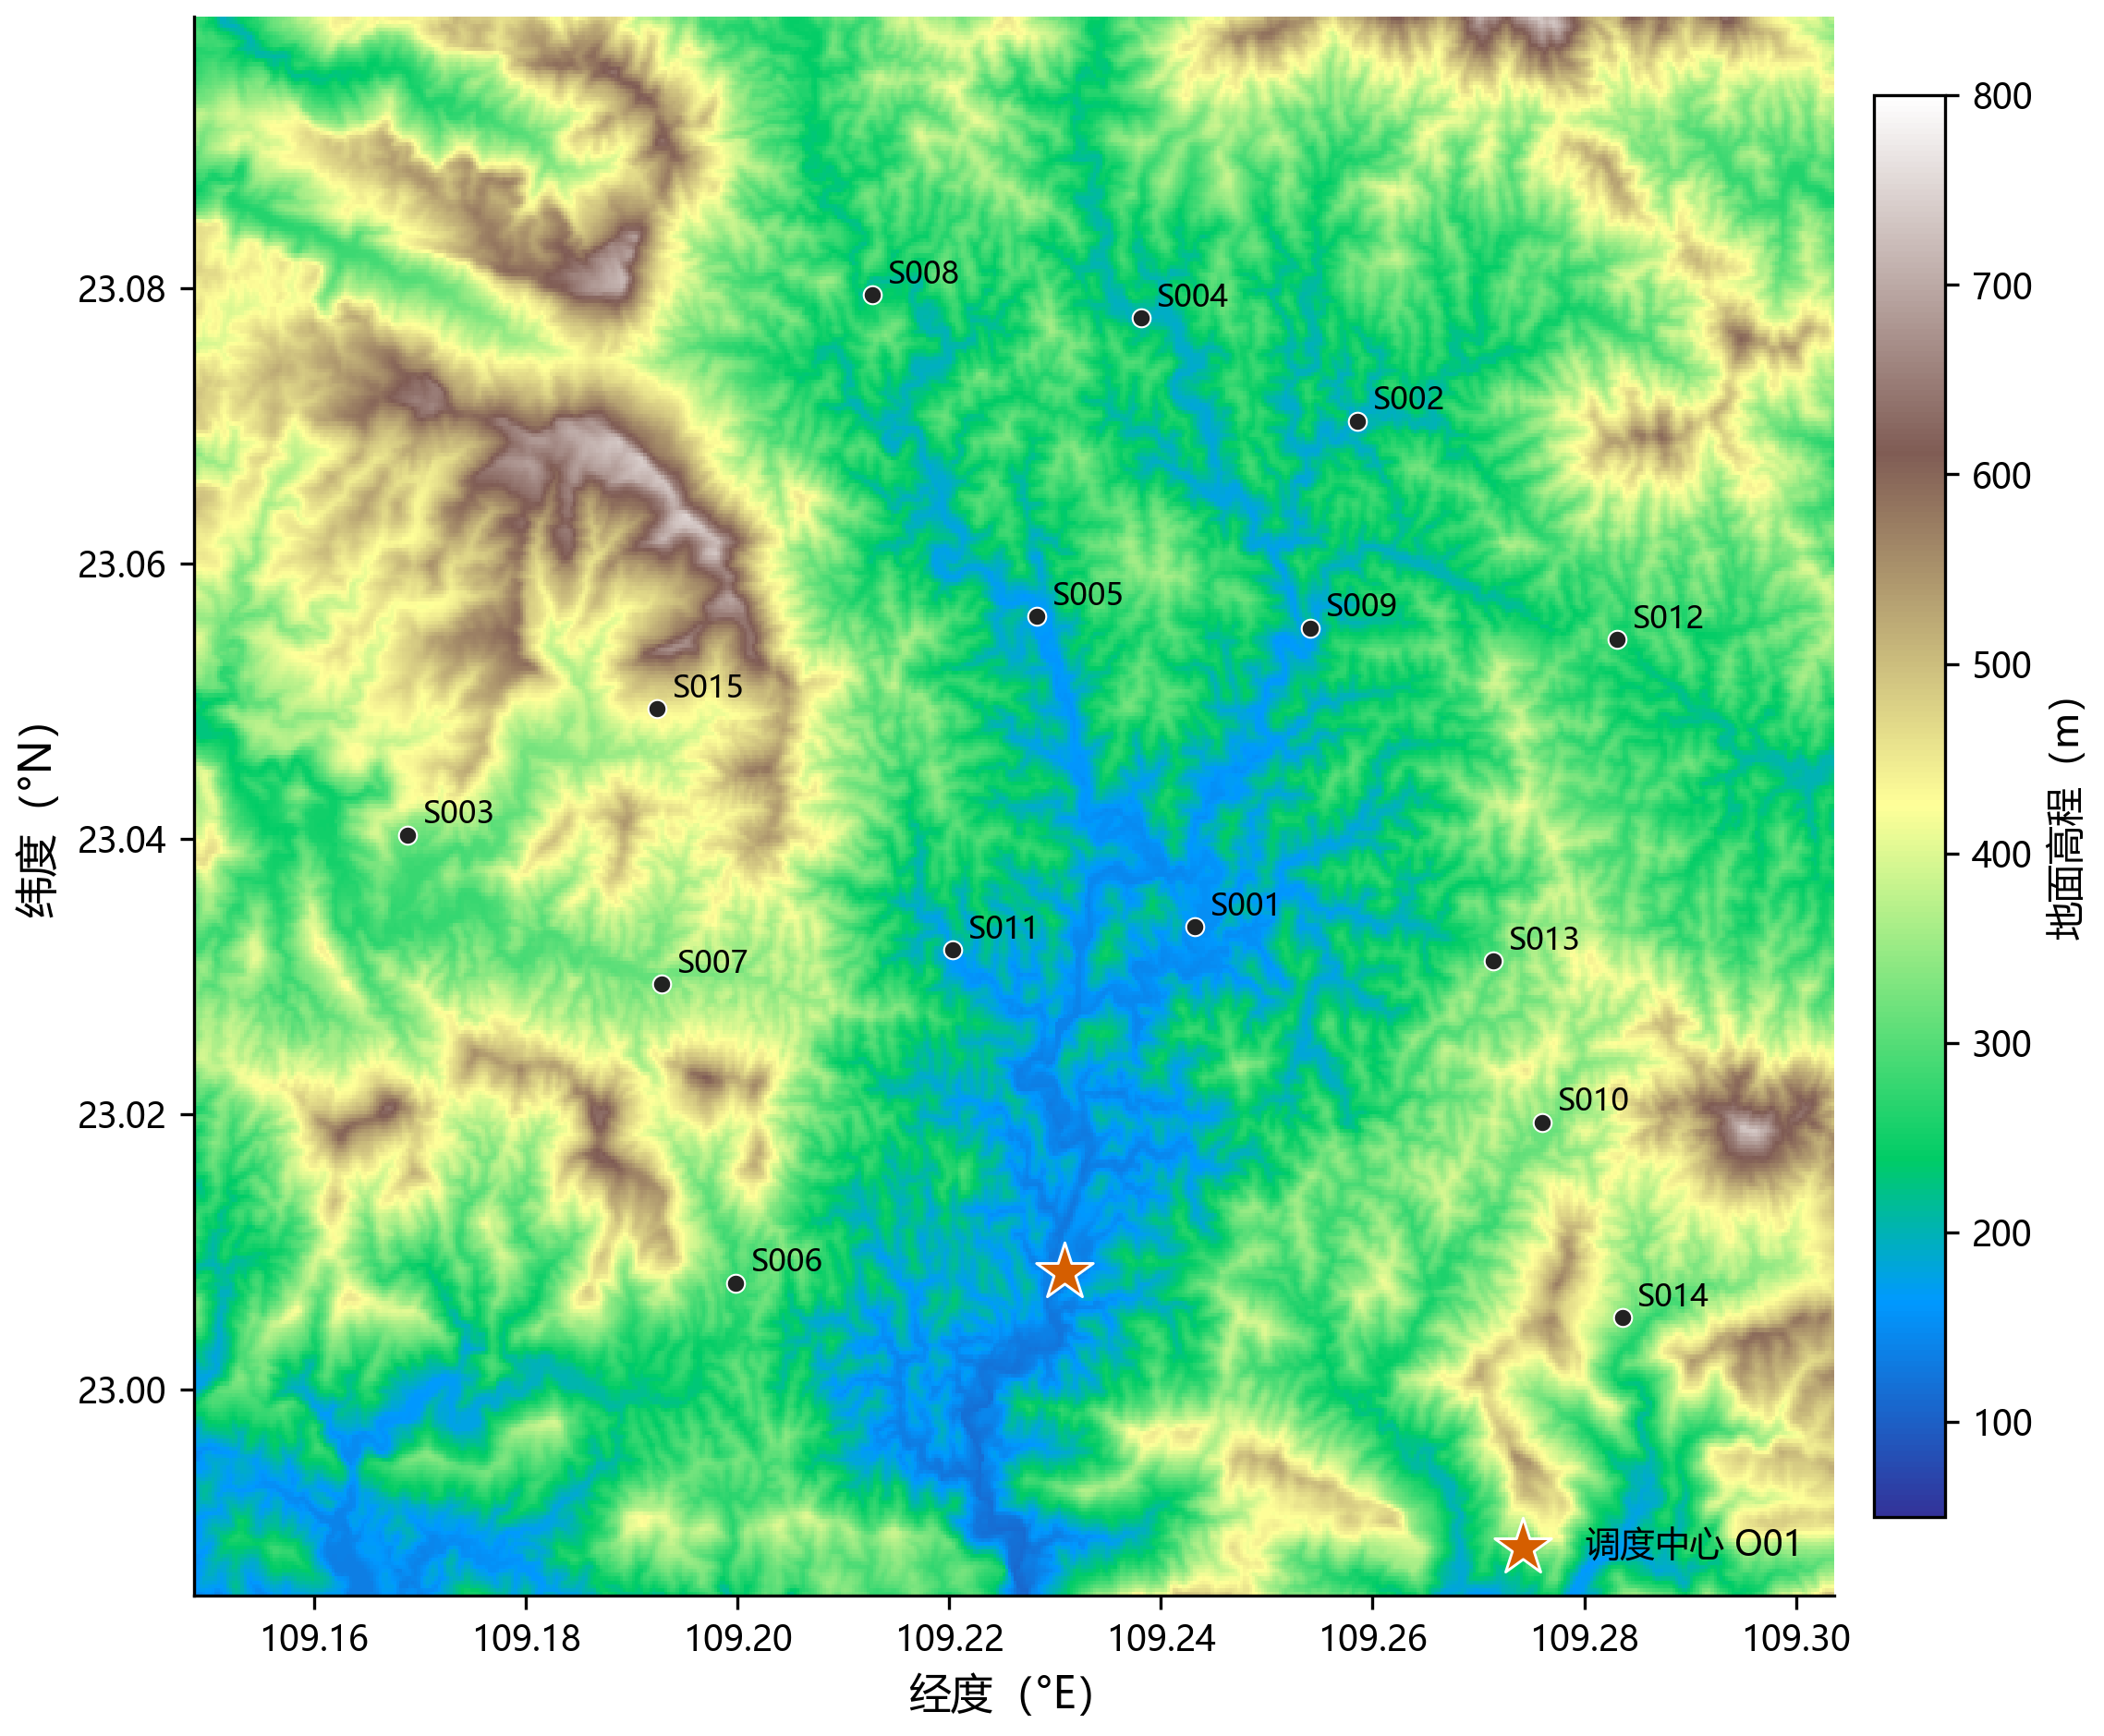
\includegraphics[width=0.78\textwidth]{figures/p1_map.png}
\caption{研究区域数字高程模型与调度节点分布（O01 为调度中心，圆点为服务区）}
\label{fig:map}
\end{figure}

本问题给出 O01 与 15 个服务区的经纬度与地面高程、30\,m 分辨率的数字高程模型、
三类运输无人机与配套电池、两架中继无人机与能源组件，以及 80 个待投运货箱
（分医疗物资、饮用水、应急食品、生活卫生用品四类，各有质量、体积与配送时限）。
题目要求在山区约束下设计无人机运输方案，并保证无人机全程通信不中断。

\subsection{问题提出}

本问题要求依次求解以下四个子问题。

\textbf{问题一：单点往返最大安全载荷与货箱组批。}针对每类运输无人机到各服务
区的单点往返任务，考虑飞行时间、载荷能耗与返航安全余量，确定单架次最大安全
载荷，并据此把各服务区货箱合理分组，给出每类机型的组批方案与架次能耗、返航
荷电状态。

\textbf{问题二：异构无人机多点多架次调度。}15 个服务区的 80 个货箱具有不同配送
时限，机队由 A、B、C 三类共 8 架无人机与 14 组共享电池组成，即 A 型 6 组、B 型 4 组、C 型 4 组。要求合理安排
各架次的任务序列、起降时刻与电池分配，使全部货箱按时送达，并尽量少用架次、
降低总能耗与总完工时间。

\textbf{问题三：通信约束下运输与中继联合调度。}无人机整个飞行过程必须与调度
中心保持通信，通信可采用直连或经悬停中继的双跳方式。中继无人机的最佳布设
位置与架次安排需结合山区地形与电波传播模型确定，并与运输调度联合优化，实现全程
无盲区且运输效率不劣化。

\textbf{问题四：任务分区与资源配置。}将 15 个服务区划分为两组与三组两种方案，
按组配备运输无人机、电池、中继无人机及能源组件等资源，考虑冗余备份，说明各
组能否独立完成保障任务，并给出资源配置方案。